% arara: indent: { overwrite : yes, files : [zigbee.tex, zigbee.bib] }
% arara: pdflatex
% arara: biber
% arara: pdflatex
% arara: pdflatex

\documentclass[a4paper,10pt,titlepage]{article}

\usepackage[utf8]{inputenc}
\usepackage{subfigure}
\usepackage[czech]{babel}
\usepackage{fontenc}
\usepackage{graphicx}
\usepackage[backend=biber, style=iso-numeric, urldate=comp]{biblatex}
\usepackage[pdftex]{hyperref}
\usepackage{url}
\usepackage{csquotes}
\usepackage[parfill]{parskip}
\usepackage[version=4]{mhchem}
\usepackage{siunitx}
\usepackage{titlesec}
\usepackage{float}

\addbibresource{zigbee.bib}

\DefineBibliographyStrings{czech}{
  url         = [Online]\addspace Dostupné z~,
}

\counterwithin{figure}{section}
\hyphenation{zig-bee}
\sisetup{detect-all}
\setcounter{secnumdepth}{4}

\titleformat{\paragraph}
{\normalfont\normalsize\bfseries}{\theparagraph}{1em}{}
\titlespacing*{\paragraph}
{0pt}{3.25ex plus 1ex minus .2ex}{1.5ex plus .2ex}

\author{Tomáš Kysela}
\title{ZigBee}
\date{\parbox{\linewidth}{\centering%
  \today\endgraf\bigskip
 Vytvořeno jako semestrální projekt pro předmět BAB34MNS\endgraf\medskip
 FEL ČVUT}}
 


\begin{document}

\pagenumbering{Alph}
\begin{titlepage}

	\maketitle

	\thispagestyle{empty}
\end{titlepage}

\pagenumbering{arabic}

\tableofcontents
\listoffigures
% \listoftables

\newpage

\section{Úvod} \label{sec:intro}
ZigBee je protokol, který navzdory zdánlivé podobnosti s~WiFi je od základu navržen primárně pro komunikaci nízkovýkonových bezdrátových zařízení ve zdravotnictví, domácí automatizaci či průmyslové automatizaci.~\cite{zigbee-tech-pres}
První specifikace vyšla v~roce 2003, v~roce 2007 pak byla částečně nahrazena specifikací ZigBee PRO, která byla následně doplněna specifikacemi ZigBee Green Power, která dovoluje Energy harvesting přímo v~ZigBee Stacku, a ZigBee Smart Energy, která slouží k~monitorování spotřeby a optimalizaci výkonů.~\cite{ecstuff4u}

\section{Princip činnosti} \label{sec:spec}

\subsection{Mesh network a typy zařízení} \label{sec:mesh}
V~běžném (například WiFi) modelu bezdrátové sítě existují tradičně dva typy zařízení, ZigBee Controller (ZC) a {ZigBee End Device} (ZED). Zatímco ZC kontroluje síť a propojuje síť s~okolním světem, ZED tradičně přijímá a odesílá informace do Controlleru. End Device může být v~síti víckrát, Controller pouze jeden. Tyto zařízení jsou zapojeny do tzv. hvězdy.

V~ZigBee je dále specifikované ještě zařízení ZigBee Router (ZR), jež funguje podobně jako End Device, avšak umí přeposílat komunikaci mezi ostatními zařízeními. Díky tomu jsme schopni dosáhnout zapojení do stromu, či do takzvané mesh sítě. Ta je výhodnější oproti stromu, jelikož lze optimalizovat cesty podle vytížení jednotlivých ZR, či kvalitě signálu vzhledem k~proměnlivým podmínkám. Také při výpadku jednqoho ZR nedojde k~výpadku celé větve.~\cite{nordic-guide}

\begin{figure}[h] \label{fig:wlan_topology}
	\centering
	
\includegraphics[width=\textwidth]{assets/topology_types.png}
	\caption[Topologie bezdrátových sítí]{Topologie bezdrátových sítí~\cite{nordic-guide}}
\end{figure}

ZigBee Router a Controller je dále typicky napojený na zdroj napájení 230V, kdy typickým Routerem je například chytrý spínač světel, Controllerem pak server. ZigBee End Device je naopak povětšinou napájené z~baterie, kdy se jedná o~všemožné senzory, hlásiče \ce{CO2} apod.

V rámci zpětné kompatibility lze přidávat ZigBee 1.0/2.0 Router zařízení do ZigBee PRO (či 3.0) sítě, avšak vzhledem ke změnám ve specifikaci lze toto zařízení používat pouze jako ZED. Stejně tak naopak lze ZigBee PRO ZR přidat do legacy ZigBee sítě, avšak pouze jako ZED.

\subsubsection{Připojení k~síti} \label{sec:joining}
Existuje několik možností připojení k~ZigBee síti. V~prvních specifikacích se používal statický klíč, který byl shodný pro všechny zařízení. Následně se přidala varianta pomocí instalačního kódu a od něj odvozeného klíče a v~revizi 23 se nově používá kryptografie s~pomocí veřejných klíčů, kde proběhne vyjednání síťového klíče.

\paragraph{Statický klíč}
Zde se využívá tzv. Trust centera (nejčastěji ZC), který centralizovaně rozhoduje, zda-li připustí nové zařízení do sítě. V případě že je využit výchozí Global Trust Center propojovací klíč, je síť dočasně vystavena případným útokům, proto byla v revizi 21 přidána možnost využití kíče odvozeného z instalačního kódu.

\begin{figure}[h] \label{fig:join_static}
	\centering
	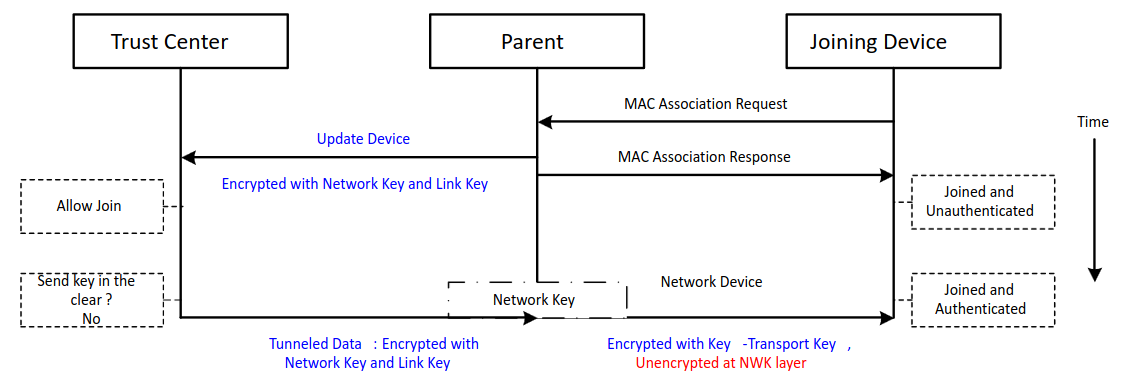
\includegraphics[width=\textwidth]{assets/join_static}
	\caption[Schéma komunikace při připojení pomocí statického klíče]{Schéma komunikace při připojení pomocí statického klíče~\cite{silabs-an1233}}
\end{figure}

\paragraph{Aktualizace klíče po připojení}
U ZigBee PRO zařízení je vyžadována aktualizace propojovacího klíče po připojení do sítě, který používají tak dlouho, dokud jsou do ní připojeni.

\paragraph{Dynamický klíč}
Od revize 23 je nově možné použít dynamické klíče, kdy je nejdříve domluveno pomocí veřejného klíče připojení a po propojení zařízení není použit jeden pevný Trust Center link key, nýbrž náhodně generovaný dynamický klíč, který se používá pro veškerou další komunikaci.

\begin{figure}[H] \label{fig:join_dynamic}
	\centering
	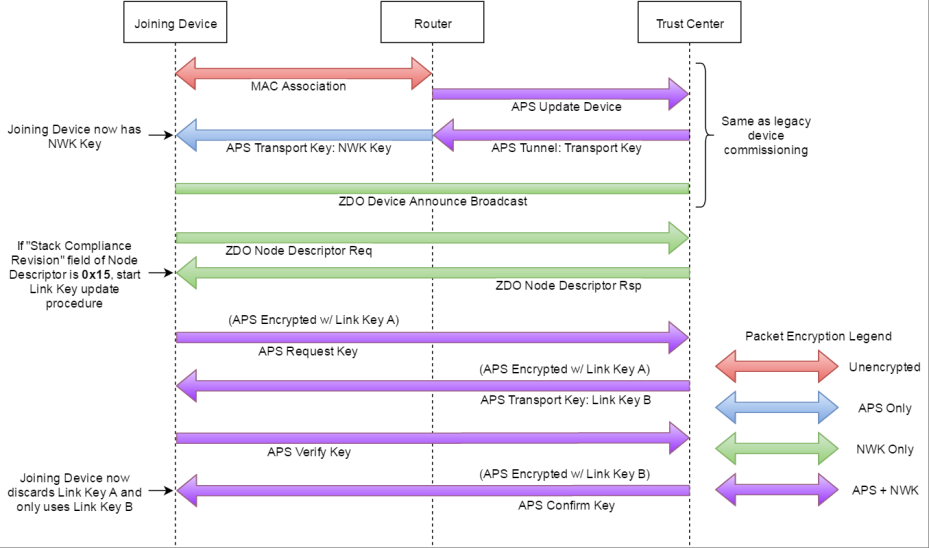
\includegraphics[width=\textwidth]{assets/join_dynamic.png}
	\caption[Schéma komunikace při připojení pomocí dynamického klíče]{Schéma komunikace při připojení pomocí dynamického klíče~\cite{ti-security}}
\end{figure}

\subsubsection{Odpojení}
Při odpojování je třeba vyslat signál pro odpojení rodiči a dětem v síti, jelikož je nutné dát jejich NLME (viz \ref{sec:NWK}) vědět, že možné cesty se změnili.

\subsubsection{Znovupřipojení}
Znovupřipojení probíhá velmi podobně jako první připojení. Změna nastává až při nastavení zapojení do sítě a jelikož si Trust Center pamatuje dřívější zařízení, je možné povolit pouze přiúojení již dříve připojených zařízení.

\subsection{Stack architektura} \label{sec:stack}
Architektura ZigBee se skláda z~několika na sobě postavených vrstev. Jelikož ZigBee vychází ze standardu IEEE~802.15.4, je tímto standardem specifikována fyzická (PHY) a Medium Access Control (MAC) vrstva. ZigBee protokol poté specifikuje síťovou (NWK) vrstvu a rámec pro aplikační vrstvu. Ten se skládá z~Podpůrné aplikační podvrstvy (APS) a ZigBee Device objektů (ZDO).~\cite{zigbee-spec23}

\begin{figure}[h] \label{fig:zb_stack}
	\centering
	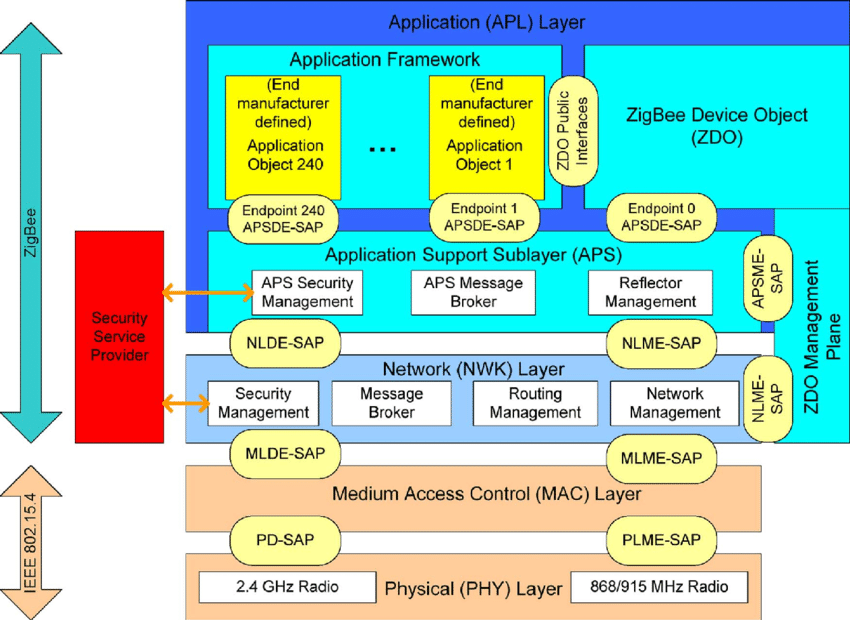
\includegraphics[width=\textwidth]{assets/stack_architecture.png}
	\caption[Schéma ZigBee Stacku]{Schéma ZigBee Stacku~\cite{5173521}}
\end{figure}

\subsubsection{PHY vrstva} \label{sec:PHY}
Tato vsrtva má na starosti fyzické vysílání signálů. Používá buď sub-GHz pásmo, konkrétně  868~MHz v~Evropě a 915~MHz v~Americe či Austrálii, nebo 2.4~GHz pásmo. Tato vrstva používá 16-QAM modulaci a přenosové rychlosti jsou až 250~kb/s pro 2.4~GHz a 915~MHz a 100~kb/s pro 868~MHz.\cite{ieee-802-15-4}

\subsubsection{MAC vrstva} \label{sec:MAC}
Účelem této vrstvy je propojení vyšších vrstev s~fyzickou vrstvou a obalení packetů tak, aby byly doručeny na správné fyzické zařízení. Označuje začátek a konec packetu, zadává adresu cílového zaříení, či opravuje drobné chyby v~přijímaných datech. MAC adresy by měli být EUI-64 definované podle IEEE~802. Mac frame je následně formátován dle obrázku \ref{fig:mac_frame}.~\cite{5173521}

\begin{figure}[h]
	\centering
	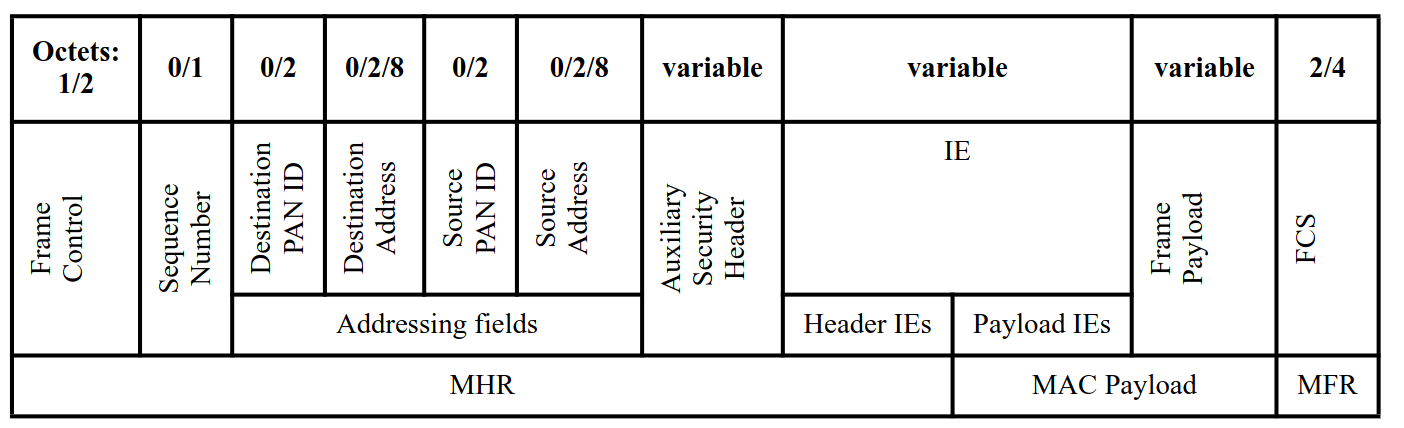
\includegraphics[width=\textwidth]{assets/mac_frame.png}
	\caption[Formát MAC Frame]{Formát MAC Frame~\cite{5173521}}
	\label{fig:mac_frame}
\end{figure}

\subsubsection{NWK vsrtva} \label{sec:NWK}
Síťová vrstva propojuje ZigBee aplikační vrstvu s~IEEE~802.15.4 MAC vrstvou. Tato vrstva se dělí na dvě části, Network Layer Data Entity (NLDE) a Network Layer Managment Entity (NLME).

NLDE se stará o~předávání application protocol data units (APDU) mezi zařízeními v~síti. Toho dosáhne za pomoci přidávání hlaviček k~APDU a následně vzhledem k~topologii sítě vyslání packetu na vhodné zařízení. Zároveň má na starost zabezpečení packetů, více v~sekci \ref{sec:security}.

NLME má na starost správu NWK vrstvy. Mezí její úkoly patří nastavení zařízení po přidání do sítě, zakládání nových sítí (pouze u~ZC), hledání vhodných cest, připojování/odpojování od sítě, adresování nových zařízení (pouze ZR a ZC), vyhledávání nových sousedů a ověřování kvality spojení se sousedy.

\subsubsection{APL vsrtva} \label{sec:APL}
Jak jsme již zmínili, tato vrstva se skládá z~ZDO a APS. ZDO je propojení samotné aplikace na ZigBee zařízení. ZDO aktivuje APS a NWK vrstvu a následně odesílá data. Dále pak čte jeden z~254 endpointů a následně předává data do aplikace. APS pak propojuje ZDO a endpointy s~NWK vrstvou. Jejím úkolem je odstranit duplikáty, rozdělení či složení zpráv delších jak maximální možný payload a spolu s~NLME se podílí na zabezpečení zpráv.

\subsection{Bezpečnost} \label{sec:security}
Jak již bylo v sekci \ref{sec:joining} zmíněno, při připojení je třeba sjednotit TC link key. Co je dále třeba je používat shodný Network key. Ten je platný pouze pro omezený počet packetů na daném zařízení a tak je možnost buď neustále kontrolovat, kolikrát již na kterém zařízení byl použit, což je nereálné, a nebo ho periodicky pomocí Truct Centera zaměňovat. Oba tyto klíče jsou používany k šifrování na NWK vrstvě. Jelikož to znamená, že každé zařízení na síti je poté schopno dešifrovat a přečíst paket, primárně za účelem případněho poslání dál, je třeba použít i šifrování na APS, kde se používají klíče, které zajišťují end-to-end šifrování.

\section{HW implementace} \label{sec:hw}
Co se týče HW implementace jedná se o vcelku jednoduché zapojení. Většina designu používá SoC, MCU, či MPU s již implementovanou většinou fyzické vrstvy, pevně programovanou MAC vrstvou a knihovnami pro NWK a APL vrstvu. Na designerovi zařízení tak povětšinou zůstávají krystaly a samotné antény. Zde je třeba jednak připravit správný timer, ale zároveň je nutné správně nastavit přizpůsobovací obvod, anténu, filtry. Nejčastěji se používá lowpass na 2.5 GHz. Samotná komunikace může používat 16-ti polohovou kvazi-ortogonální modulaci, avšak vždy se jedná o poloduplex.

\begin{figure}[h] \label{fig:rf-ext}
	\centering
	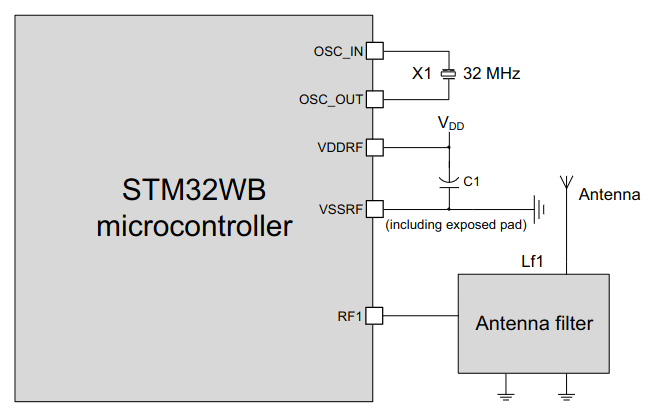
\includegraphics[width=0.75\textwidth]{assets/rf_external.png}
	\caption[Vzorové zapojení vnějších komponent u STM32WB]{Vzorové zapojení vnějších komponent u STM32WB~\cite{stm32wb}}
\end{figure}


Mezi významené výrobce SoC a MCU se řadí Texas Instruments (TI CC2530Fxx), či ST (ST STM32WBx5). Od výrobce je často dodávána i knihovna pro implementaci SW.

\begin{figure}[H] \label{fig:rf-int}
	\centering
	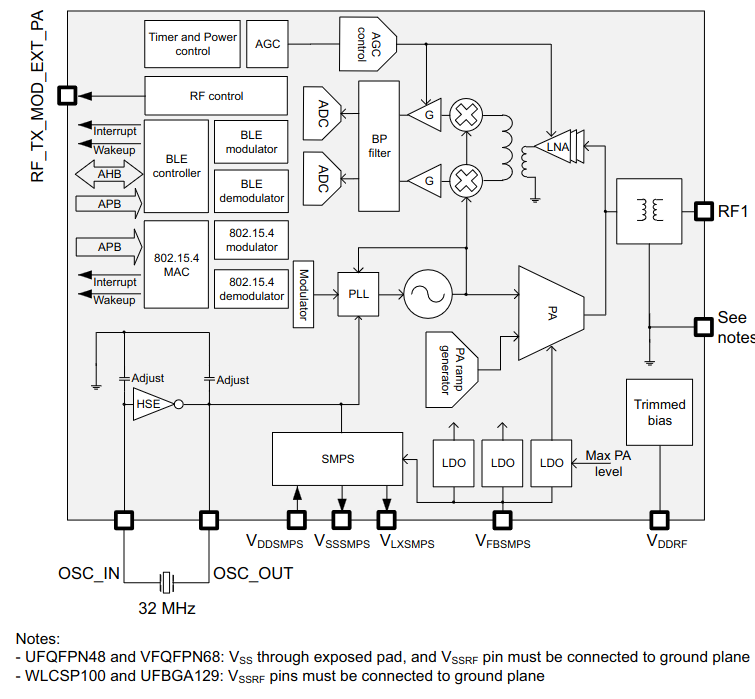
\includegraphics[width=0.75\textwidth]{assets/rf_inner.png}
	\caption[Vnitřní zapojení RF bloku u STM32WB]{Vnitřní zapojení RF bloku u STM32WB~\cite{stm32wb}}
\end{figure}

\section{Využití}
Mezi typické využití ZigBee na 2.4 GHz patří chytré spínače, žárovky, zásuvky. Tyto zařízení fungují také jako ZigBee Routery. Dalším využitím jsou například meteostanice, senzory plynu, světla, pohybu. Tyto zařízení jsou nejčastěji ZigBee End Device. Mezi průmyslové využití patří monitoring strojů ve výrobě, sledování vhodných podmínek pro staření produktů, potravin a mnoho dalšího.

Sub-GHz využití je pak nejčastěji připojení venkovních zařízení do ZigBee sítě, například monitorování solárních panelů, ovládání vjezdové brány apod.

\section{Závěr}
Connectivity Standards Alliance v čele s firmami jako je Schneider Electrics, ST, TI, či IKEA tvoří stále se vyvíjející moderní standard, jež má významnou roli na poli nízkovýkonových vnitřních sítí pro IoT aplikace.

\section{Zdroje}
\nocite{*}
\printbibliography[heading=none]
\end{document}
